\section{Grundbegriffe}

\begin{frame}
    \frametitle{\insertsection}
    \textbf{Allgemeine Begriffe}\\
    \begin{definition}[Messen]
        \centering
        Messen bedeutet das quantitative Erfassen einer Größe,\\
        der sogenannten Messgröße.
    \end{definition}
    %
    \begin{definition}[Messtechnik]
        \centering  
        Messtechnik ist die objektive, reproduzierbare und quantitative Erfassung einer physikalischen Größe
    \end{definition}
    \textbf{Dabei bedeutet} (nach \cite{muhl2017})\\
    \begin{itemize}
        \item Objektiv: unabhängig von Sinnesorganen des Menschen
        \item Reproduzierbar: wiederholbar und kontrollierbar
        \item Quantitativ: mit einem Zahlenwert versehen
    \end{itemize}
\end{frame}


% new idea
\begin{frame}
    \frametitle{\insertsection}
    \begin{definition}[Messgröße (Measurand) \cite{muhl2017}]
        \centering
        Physikalische Größe, die durch die Messung bestimmt werden soll.
        \note[item]{Messgröße: Dies kann in allgemeiner Form, beispielsweise die Energie oder der Widerstandswert oder auch eine bestimmte Größe sein wie die Spannung einer speziellen Batterie oder der Gleichstromwiderstandswert eines konkreten Leiters}
    \end{definition}

    \begin{definition}[Messgerät (Measuring Instrument) \cite{muhl2017}]
        \centering
        Das Gerät, das für die Messung einer Größe vorgesehen ist.
        \note[item]{Messgerät: Das Messgerät kann eine Anzeige enthalten oder die Messgröße umformen oder bearbeiten wie beispielsweise ein Strom-Spannungswandler oder Messverstärker.}
    \end{definition}

    \begin{definition}[Messeinrichtung (Measuring System) \cite{muhl2017}]
        \centering
        Ein System, bestehend aus einem oder mehreren Messgeräten zusammen mit für die Messung notwendigen, zusätzlichen Einrichtungen wie z. B. Energieversorgung.
        \note[item]{Messeinrichtung: Beispiele sind ein Digitalvoltmeter (DVM), ein Widerstandsmessplatz oder eine Kalibriereinrichtung.}
    \end{definition}
\end{frame}

% old frame from PowerPoint
\begin{frame}
    \frametitle{\insertsection}
    \begin{itemize}
        \item Messgröße (Measurand)
        \item Messgerät (Measuring Instrument)
        \item Messeinrichtung (Measuring System)
        \item Messgrößenaufnehmer (Sensor)
        \item Messwert (Measured Value) $x_i$
        \item Wahrer Wert (True Value) $x_{\text{w}}$
        \item Tatsächlicher Merkmalswert, ist in der Regel aber nur ein ideeller Wert, weil praktisch nicht ermittelbar. Typischerweise können nicht alle beitragen Faktoren vermieden werden.
        \item Richtiger Wert (Conventional True Value)
        \item Wert für Vergleichszwecke, dessen Abweichung vom wahren Wert für den Vergleichszweck als vernachlässigbar betrachtet wird.
        \item Messabweichung (Error of Measurement) $e$
        \item Messergebnis minus wahrer Wert der Messgröße.
        \item Messergebnis (Result of Measurement)
        \item Messunsicherheit (Uncertainty of Measurement) %u%
        \item Geschätzter Betrag zur Kennzeichnung eines Wertebereichs, innerhalb dessen der Bezugswert liegt.
    \end{itemize}
\end{frame}


\section{Werte und Einheiten}

\begin{frame}
    \frametitle{\insertsection}
    \begin{itemize}
        \item Messergebnis
        \begin{itemize}
            \item Größenwert = Zahlenwert $\cdot$ Einheit
            \item Ohne Einheit nicht sinnvoll
        \end{itemize}
        \item Ursprung: Einheiten aus Erfahrungswelt
        \begin{itemize}
            \item Elle
            \item Fuß
            \item Regional unterschiedlich
        \end{itemize}
        \item Ziel der Metrologie (Lehre und Wissenschaft vom Messen, von den\\ 
              Maßsystemen und deren Einheiten):
              \begin{itemize}
                  \item Einheitliche Einheiten
                  \item Frei von äußeren Einflüssen (Zeit, Ort, Mensch)
                  \item Jederzeit reproduzierbar durch Experimente nachvollziehbar
              \end{itemize}
    \end{itemize}

\end{frame}


\section{SI Einheiten}

\begin{frame}
    \frametitle{\insertsection}
    \begin{itemize}
        \item SI: „Système international d`unités“ (Internationales Einheitensystem)
        \item sieben standardisierte Basis-Einheiten
        \item alle anderen gebräuchlichen Einheiten daraus ableitbar    
    \end{itemize}
    \vfill
    \begin{table}
        \centering
        \begin{tabular}{lccc}
            Basisgröße & Formelzeichen & Basiseinheit & Einheitszeichen\\
            \hline
            Länge & $l$ & Meter & \si{\meter}\\
            Masse & $m$ & Kilogram & \si{\kilo\gram}\\
            Zeit & $t$ & Sekunde & \si{\second}\\
            Stromstärke & $I$ & Ampere & \si{\ampere}\\
            Temperatur & $T$ & Kelvin & \si{\kelvin}\\
            Lichtstärke & $I$ & Candela & \si{\candela}\\
            Stoffmenge & $n$ & Mol & \si{\mol}
        \end{tabular}
        \caption{Die sieben SI Basiseinheiten.}
    \end{table}
\end{frame}

\section{Einheitenpräfixe}

\begin{frame}
    \frametitle{\insertsection}
    \begin{itemize}
        \item Messergebnisse können großen Wertebereich abdecken
        \item Abkürzungen durch Namen für Zehnerpotenzen
    \end{itemize}
    \vfill
    \begin{table}
        \begin{tabular}{lcc}
            Name & SI-Präfix & Wert\\
            \hline
            Dezi- & \si{\deci\relax} & $10^{-1}$\\
            Zenti- & \si{\centi\relax} & $10^{-2}$\\
            Milli- & \si{\milli\relax} & $10^{-3}$\\
            Mikro- & \si{\micro\relax} & $10^{-6}$\\
            Nano- & \si{\nano\relax} & $10^{-9}$\\
            Pico- & \si{\pico\relax} & $10^{-12}$\\
            Femto- & \si{\femto\relax} & $10^{-15}$\\
            Atto- & \si{\atto\relax} & $10^{-18}$\\
        \end{tabular}
        \hspace{1cm}
        \begin{tabular}{lcc}
            Name & SI-Präfix & Wert\\
            \hline
            Deka- & \si{\deca\relax} & $10^{1}$\\
            Hekto- & \si{\hecto\relax} & $10^{2}$\\
            Kilo- & \si{\kilo\relax} & $10^{3}$\\
            Mega- & \si{\mega\relax} & $10^{6}$\\
            Giga- & \si{\giga\relax} & $10^{9}$\\
            Tera- & \si{\tera\relax} & $10^{12}$\\
            Peta- & \si{\peta\relax} & $10^{15}$\\
            Exa- & \si{\exa\relax} & $10^{18}$\\
        \end{tabular}
        \caption{Die Präfixe im SI}
    \end{table}
\end{frame}

\section{Präzision und Genauigkeit}

\begin{frame}
    \frametitle{\insertsection}
    \begin{columns}[c, onlytextwidth]
        \begin{column}{0.6\textwidth}
            \textbf{Genauigkeit}
            \begin{itemize}
                \item Abweichung eines Messwerts vom wahren Wert
                \item Auch Richtigkeit oder Werttreue genannt
            \end{itemize}
            \textbf{Präzision}
            \begin{itemize}
                \item Möglichst kleine Abweichungen der gemessenen Werte voneinander bei konstanten Gegebenheiten
                \item Werte müssen nicht richtig sein
            \end{itemize}
            \textbf{Reproduzierbarkeit}
            \begin{itemize}
                \item Messabweichungen bei wiederholtem Aufbau der Messgegebenheiten
                \item Entspricht in etwa einer Präzision im dynamischen Fall
            \end{itemize}
        \end{column}
        \begin{column}{0.4\textwidth}
            \begin{figure}
                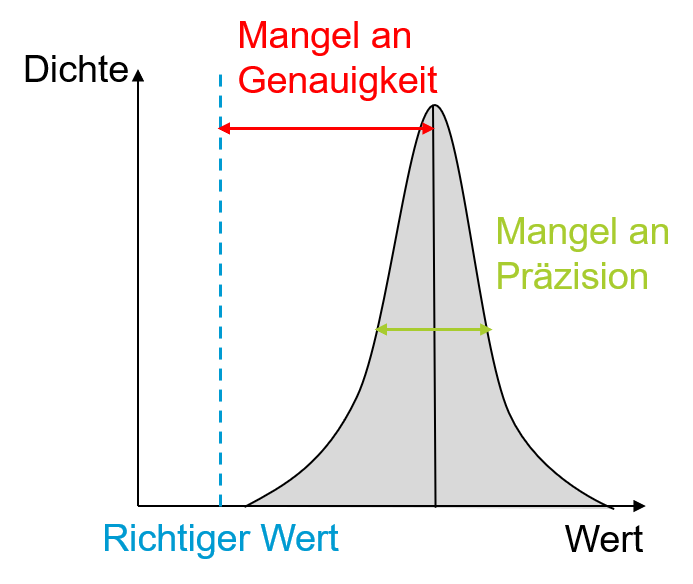
\includegraphics[width=\columnwidth]{fig/slides_messtechnik1_ws21_18}
                \caption{Illustration: Genauigkeit vs. Präzision}
            \end{figure}
        \end{column}
        \end{columns}
\end{frame}

\begin{frame}
    \frametitle{DIN 55 350-13 Begriffe der Qualitätssicherung und Statistik }
    \note[item]{Titelzusatz: Begriffe zur Genauigkeit von Ermittlungsverfahren und -ergebnissen (Juli 1987) }
    \begin{figure}
        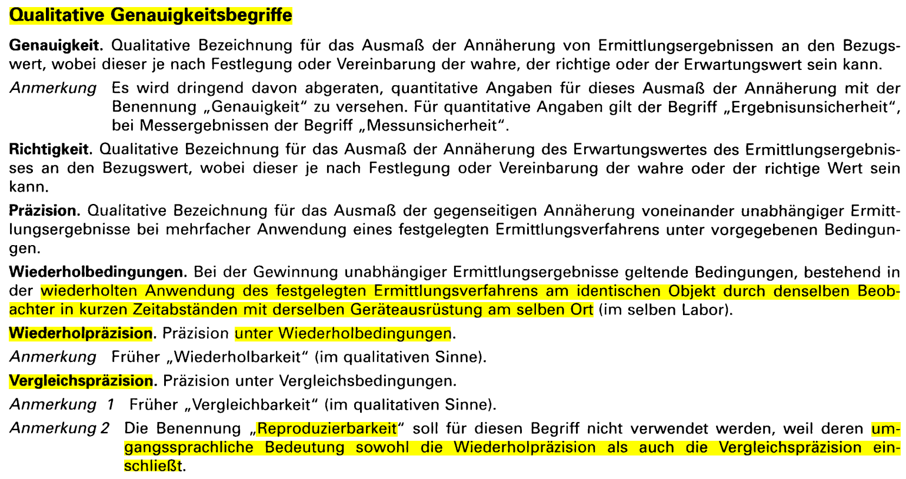
\includegraphics[width = \columnwidth]{content/grundlagen_des_messens/fig/slides_messtechnik1_ws21_19.png}
    \end{figure}
\end{frame}

\section{Abgrenzung Grundbegriffe}

\begin{frame}
    \frametitle{\insertsection}
    \begin{columns}[onlytextwidth]
       \begin{column}{0.5\textwidth}
           \begin{itemize}
               \item Wandler
               \begin{itemize}
                   \item Wandelt eine physikalische Größe in eine andere
                   \item Z.B. Mikrofon: mechanische Schwingung in elektrische Schwingung
                   \item \textsl{Bezeichnung\\"Spannungswandler" ist in diesem Kontext irreführend}
               \end{itemize}
               \item Umsetzer
               \begin{itemize}
                   \item Setzt eine physikalische Größe in eine andere Repräsentation derselben Größe um
                   \item Z.B. Transformator
               \end{itemize}
           \end{itemize}
       \end{column}
       \begin{column}{0.5\textwidth}
        \begin{itemize}
            \item Kontinuierlich
            \begin{itemize}
                \item Größe ist stetig über Wertebereich darstellbar
            \end{itemize}
            \item Diskontinuierlich
            \begin{itemize}
                \item Unstetiger Wertebereich der Größe
            \end{itemize}
        \end{itemize}
    \end{column}
    \end{columns}
\end{frame}

\begin{frame}
    \frametitle{\insertsection}
    \begin{itemize}
        \item Analog
        \begin{itemize}
            \item Kontinuierlich in Wert oder Zeit
            \item Alltägliche, in der Natur vorherrschende Darstellung
        \end{itemize}
        \item Digital 
        \begin{itemize}
            \item Diskret in Wert und Zeit
            \item Abbildung auf binäre Repräsentation
            \item Binäre Wert ist im Verhältnis zum Maximalwert zu interpretieren
            \item Maximalwert nicht aus binärem Wert ersichtlich, sondern über Referenz definiert
            \item Diskretisierung im Zeitbereich
            \begin{itemize}
                \item Name: Abtastung
                \item Bei Einhalten des Abtasttheorems analoger Wert fehlerfrei rekonstruierbar
            \end{itemize}
            \item Diskretisierung im Wertebereich
            \begin{itemize}
                \item Name: Quantisierung
                \item Quantisierungsfehler immer unvermeidbar
            \end{itemize}
        \end{itemize}
    \end{itemize}
\end{frame}

\section{Quantisierungsfehler}

\begin{frame}
    \frametitle{\insertsection}
    \begin{columns}[c, onlytextwidth]
        \begin{column}{0.5\textwidth}
            \begin{itemize}
                \item Mit jedem zusätzlichen Bit halbiert sich der Quantisierungsfehler
                \begin{itemize}
                    \item Anzahl der Stufen $\mathcal{N}$ verdoppelt sich
                    \item Stufenbreite halbiert sich
                \end{itemize}
                \item Signalqualität steigt mit / 6dB Bit\\
                   \[
                      S_{dB} = 20 dB \cdot \lg{U_{e,eff} \over\displaystyle U_{r,eff}} 
                    \]
                    \[
                        = 6 dB \cdot \log_2{ {U_{e,eff} \over\displaystyle U_{r,eff} }}
                    \]
                    \[
                        =\mathcal{N} \cdot 6dB + 1,76 dB 
                    \]
                    \[
                        \approx \mathcal{N} \cdot 6dB
                    \]
            \end{itemize}
        \end{column}
        \begin{column}{0.5\textwidth}
            \begin{figure}
                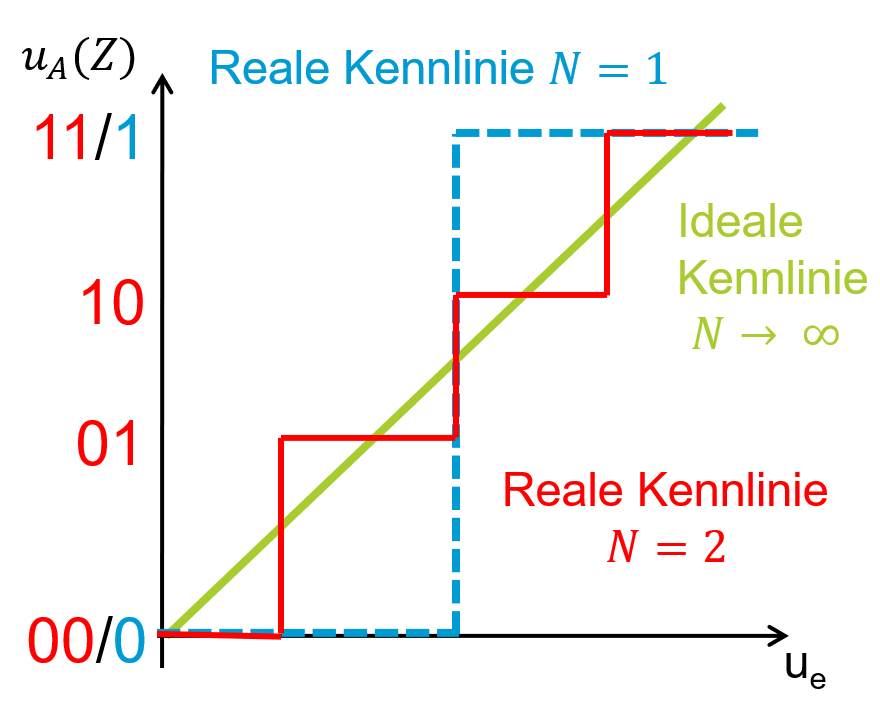
\includegraphics[width=0.7\columnwidth]{fig/slides_messtechnik1_ws21_22_1.PNG}
                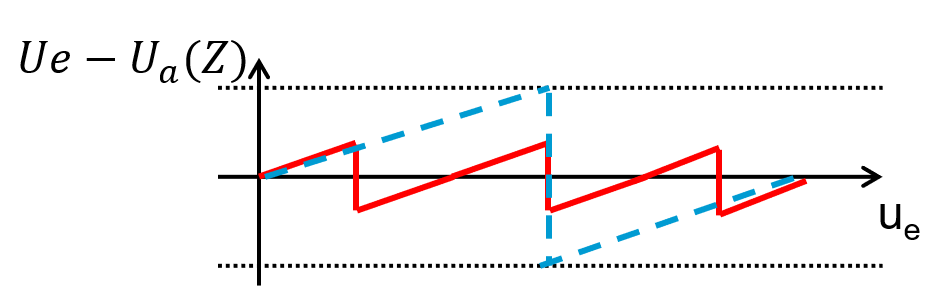
\includegraphics[width=\columnwidth]{content/grundlagen_des_messens/fig/slides_messtechnik1_ws21_22_2.PNG}
                \caption{Illustration: Quantisierungsfehler }
            \end{figure}
        \end{column}
    \end{columns}
\end{frame}

\section{Abgrenzung Grundbegriffe}

\begin{frame}
    \frametitle{\insertsection}
    \begin{itemize}
        \item Ausschlag
        \begin{itemize}
            \item Messgröße in (möglichst) proportionalen Ausschlag umwandeln
            \item Z.B. Zeigerinstrument
            \item Entzug von Energie aus dem Messobjekt → Rückwirkung
        \end{itemize}
        \item Kompensation
        \begin{itemize}
            \item Erzeugen einer Kompensationsgröße aus Hilfsenergie
            \item Regelstrecke: Differenz zwischen Messgrößen und Kompensation wird zu null geregelt
            \item Ausgabe des Kompensationssignals als Ergebnis
        \end{itemize}
    \end{itemize}
\end{frame}

\begin{frame}
    \frametitle{\insertsection}
    \begin{itemize}
        \item Direkt
        \begin{itemize}
            \item Unmittelbar mit Messkörpern derselben physikalischen Dimension vergleichen
            \item Z.B. Voltmeter
        \end{itemize}
        \item Indirekt
        \begin{itemize}
            \item Messgröße zunächst in proportionale Zwischengröße umwandeln
            \item Zusammenhang zwischen Zwischengröße und Messgröße muss bekannt sein
            \item Z.B. elektrische Leistung über Temperatur am Widerstand bestimmen
        \end{itemize}
    \end{itemize}
\end{frame}

\section{Kalibrieren}
\begin{frame}
    \frametitle{\insertsection}
    \begin{itemize}
        \item Zuverlässige Feststellung der Abweichung eines Messgeräts vom Wert
        \item Ermittlung über eine Referenz oder Referenz-Messgerät
        \begin{itemize}
            \item Name: Normal
            \item Muss in der Regel selbst auch selbst Kalibriert werden
        \end{itemize}
        \item Nationale Normungsinstitute
        \begin{itemize}
            \item PTB - Physikalisch-Technische Bundesanstalt, Deutschland
            \item NPL - National Physical Laboratory, Großbritannien
            \item NIST - National Institute for Standards and Technology, USA
            \item NRLM - National Research Laboratory, Japan
        \end{itemize}
    \end{itemize}
\end{frame}

\begin{frame}
    \frametitle{\insertsection}
    \begin{itemize}
        \item Hierachie-Ebenen
        \begin{itemize}
            \item Internationale Normale: international anerkannte Referenzgrößen, z.B. UrKilogramm
            \item Primärnormale: bei nationalen Instituten aufbewahrt und gegeneinander vergleichbar, z.B. Cäsium-Atomuhr
            \item Sekundärnormale: Als Referenz bei Kalibrierstellen vorgehaltene Normale, werden nur bei Rekalibrierung verwendet, z.B. präzise Uhr
            \item Gebrauchsnormale: Werden real eingesetzt
        \end{itemize}
        \item Kalibrierstandards oder Normale sind wertvoll
        \begin{itemize}
            \item Sollten nur zur Kalibration und Validierung verwendet werden
            \item Sind nicht für den Alltagseinsatz gedacht
        \end{itemize}
    \end{itemize}
\end{frame}

\section{Informationsträger im Messsignal}
\begin{frame}
    \frametitle{\insertsection}
    \begin{columns}
        \begin{column}{0.6\textwidth}
            \begin{itemize}
                \item Elektrische Messtechnik
                \begin{itemize}
                    \item Information als wahrnehmbarer Parameter auf Signalträger verhanden
                    \item Eng verknüpft mit dem Begriff Modulation
                \end{itemize}
                \item Analoge Informationsparameter
                \begin{itemize}
                    \item Amplitude
                    \item Frequenz
                    \item Phase 
                \end{itemize}
                \item Repräsentation über digitale Darstellung möglich 
                \begin{itemize}
                    \item Pulscodemodulation: \\Binärzahl $\rightarrow$  Zeit \&  Wert diskret
                    \item Pulsdauermodulation: \\Messwert $\sim $ Pulsdauer \\ $\rightarrow $ Zeit analog, ein Wert
                \end{itemize}
            \end{itemize}
            
        \end{column}
        \begin{column}{0.4\textwidth}
            \begin{figure}
                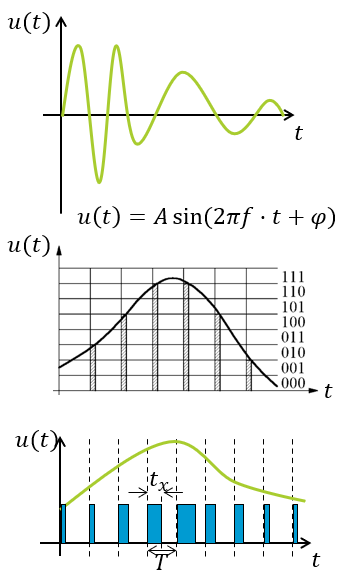
\includegraphics[height = 6cm, width=0.9\columnwidth]{fig/slides_messtechnik1_ws21_28.PNG}
                \caption{Illustration: Modulation}
            \end{figure} 
            
        \end{column}
    \end{columns}
\end{frame}

